%\title{LaTeX Portrait Poster Template}
%%%%%%%%%%%%%%%%%%%%%%%%%%%%%%%%%%%%%%%%%
% a0poster Portrait Poster
% LaTeX Template
% for Humboldt-University Berlin 
% created by Patrick Jähnichen (patrick.jaehnichen@hu-berlin.de) on 29/6/2016
% licensed under CC BY-NC-SA 3.0 (http://creativecommons.org/licenses/by-nc-sa/3.0/)
%
% The a0poster class was created by:
% Gerlinde Kettl and Matthias Weiser (tex@kettl.de)
% 
% This template has been downloaded from:
% http://www.LaTeXTemplates.com
%
% License:
% CC BY-NC-SA 3.0 (http://creativecommons.org/licenses/by-nc-sa/3.0/)
%
%%%%%%%%%%%%%%%%%%%%%%%%%%%%%%%%%%%%%%%%%

%----------------------------------------------------------------------------------------
%	PACKAGES AND OTHER DOCUMENT CONFIGURATIONS
%----------------------------------------------------------------------------------------

\documentclass[a1,portrait]{a0poster}

\usepackage{multicol} % This is so we can have multiple columns of text side-by-side
\columnsep=.2\linewidth % This is the amount of white space between the columns in the poster
\columnseprule=2pt % This is the thickness of the black line between the columns in the poster

\usepackage[svgnames]{xcolor} % Specify colors by their 'svgnames', for a full list of all colors available see here: http://www.latextemplates.com/svgnames-colors

\usepackage{times} % Use the times font
%\usepackage[margin={5cm, 5cm, 1cm, 1cm}]{geometry}

%\usepackage{palatino} % Uncomment to use the Palatino font

\usepackage{graphicx} % Required for including images
\graphicspath{{figures/}} % Location of the graphics files
\usepackage{booktabs} % Top and bottom rules for table
\usepackage{amsfonts, amsmath, amsthm, amssymb} % For math fonts, symbols and environments
\usepackage{wrapfig} % Allows wrapping text around tables and figures

\usepackage{subfig}
%----------------------------------------------------------------------------------------
%	HU COLORS 
%----------------------------------------------------------------------------------------
\RequirePackage{hucolors}

\usepackage[font={footnotesize, color=hu_green, bf}, figurename=Fig., labelfont={bf}]{caption}% Required for specifying captions to tables and figures

\usepackage{titlesec}
\begin{document}
	\titlespacing*{\section}
	{0pt}{1.5ex}{1.3ex}

%----------------------------------------------------------------------------------------
%	POSTER HEADER 
%----------------------------------------------------------------------------------------

% The header is divided into two boxes:
% The first is 75% wide and houses the title, subtitle, names, university/organization and contact information
% The second is 25% wide and houses a logo for your university/organization or a photo of you
% The widths of these boxes can be easily edited to accommodate your content as you see fit
\setlength{\linewidth}{1450pt}

\begin{minipage}[t]{0.75\linewidth}
\huge \color{hu} \textbf{Bootstrapping the Support Vector Machine} \color{Black}\\[0.5cm] % Title
\large \textbf{Thomas Goerttler, Christian Koopmann, Patricia Craja}\\[0.5cm] % Author(s)
\large Department of Computer Science,\\
\large Machine Learning Group\\[0.4cm] % University/organization
\large Humboldt-University of Berlin, Germany\\
\normalsize \texttt{thomas.goerttler@gmail.com, c.k.e.koopmann@gmail.com, Patricia.craja@gmx.de}\\
\end{minipage}
%
\begin{minipage}[t]{0.24\linewidth}
\vspace{-50pt}
\raggedleft

\includegraphics[width=\linewidth]{husiegel_bw.pdf}%\hspace{\linewidth}
\vfill
\end{minipage}

\vspace{1cm} % A bit of extra whitespace between the header and poster content
\color{hu}
\noindent\makebox[\linewidth]{\rule{\paperwidth}{2pt}}
\color{Black}
%----------------------------------------------------------------------------------------
%\the\linewidth
\begin{multicols}{3} % This is how many columns your poster will be broken into, a portrait poster is generally split into 2 columns

%----------------------------------------------------------------------------------------
%	ABSTRACT
%----------------------------------------------------------------------------------------

\color{hu} % HU color for the abstract

\begin{abstract}
\footnotesize
The goal of this project is the analysis of the variance of Support Vector Machines (SVMs) and the relationship between this variance and other important aspects of the SVM for both Linear and Gaussian Kernels. We calculate the variance of SVMs using the minimal distance of prediction points to the decision boundary by applying the bootstrap method.  
\end{abstract}
%----------------------------------------------------------------------------------------
%	INTRODUCTION
%----------------------------------------------------------------------------------------

\footnotesize

\color{Black} % Black color for the rest of the content

\section*{Introduction}

In contrast to probabilistic classifiers which provide classification with a degree of certainty, SVMs only predict the most likely class that the sample should belong to.  

We apply the bootstrapping method to the SVM algorithm, i.e. drawing random training samples with replacement from the full training data set to train different SVMs. Through the repeated calculation of the predictions of the test data set we can estimate the prediction variance, which is an indicator of the degree of certainty of the SVM. 

Since Predictions might be identical across all bootstrap samples, we use a real valued substitute: the minimal distance of each prediction point to the decision boundary (Figure 1\label{fig1}). 
\begin{center}\vspace{1cm}
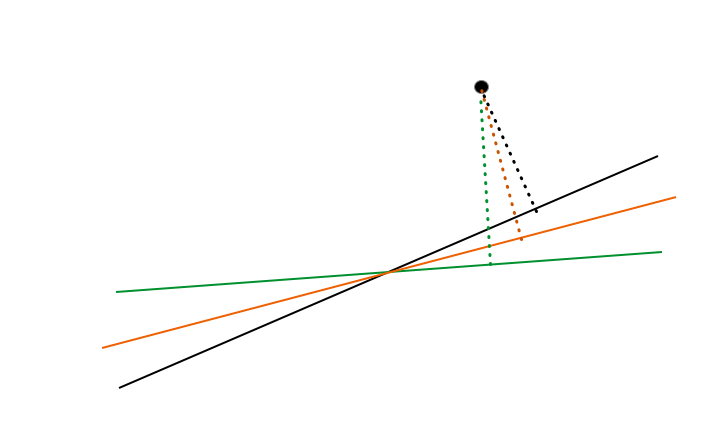
\includegraphics[width=0.8\linewidth]{abb/distances.jpg}
\captionof{figure}{The minimal distance of a prediction point to each hyperplane is considered.}
\end{center}\vspace{1cm}

%----------------------------------------------------------------------------------------
%	MATERIALS AND METHODS
%----------------------------------------------------------------------------------------

\section*{Implementation}
\subsection*{Bootstrapping}
In order to calculate the variance of the predictions we use bootstrap samples. We first train the SVM on the full training data and will call this SVM the \textit{Full SVM}. Then we draw $N$ random bootstrap samples(\cite{christmann_bootstrap_2013}) and train $N$ separate SVMs on each bootstrap sample so we get $N$ different set of predictions on the test data. Figure 2 \label{fig2} shows, that the variance decreases with better separation and more data.

The $n$ distances of each point in the test data set from the decision boundary can be seen as random variables. For the $N$ SVMs we obtain $N$ different values of these random variables and can calculate their variance. We take the average of these $n$ variances as an indicator for the variance of the \textit{Full SVM}.

\begin{center}\vspace{1cm}
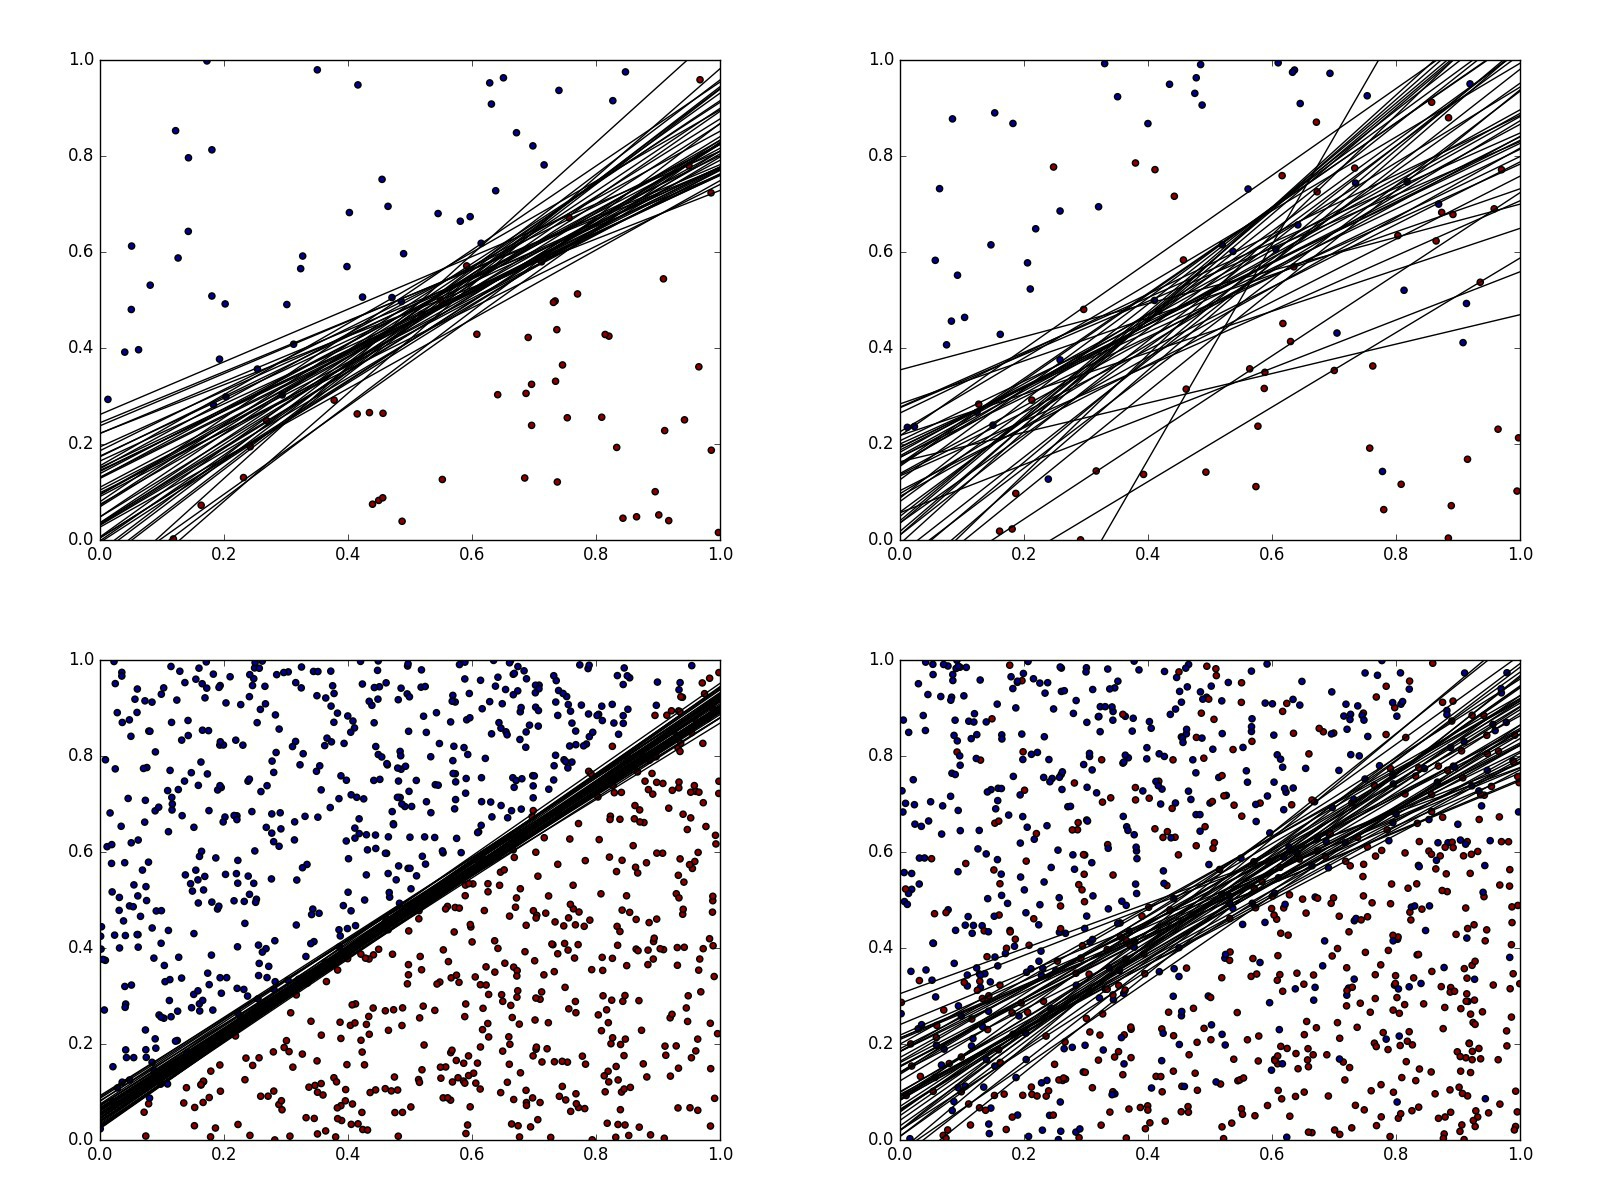
\includegraphics[width=1\linewidth]{abb/pic.jpg}
\captionof{figure}{100 hyperplanes plotted based on samples,(a) and (c) use perfectly separated data, (b) and (d) not. In (a) and (b) use 100 observations in the training data,(c) and (d) 1000.}
\label{fig3}
\end{center}\vspace{1cm}


\subsection*{Data Simulation}
We draw $n$ observations for each of the input variables $x$ from a normal distribution and use the Hyperplane-Approach: labels calculated using the formula $y= sign(c+ w^T x + error)$.
To change the number of support vectors of a data set the variance of the error is modified, while the intercept controls the balance of the data set.

%	RESULTS 
%----------------------------------------------------------------------------------------

\section*{Results}
In this section we will show how the prediction variance is correlated with the regularization parameter $C$, the balance of the training data set and the number of support vectors of the original \textit{Full SVM}. The size of each data set will be denoted by $n$, the number of bootstrap replications by $N$. The first graph corresponds to the Linear, the second to the Gaussian Kernel.

\begin{center}\vspace{1cm}
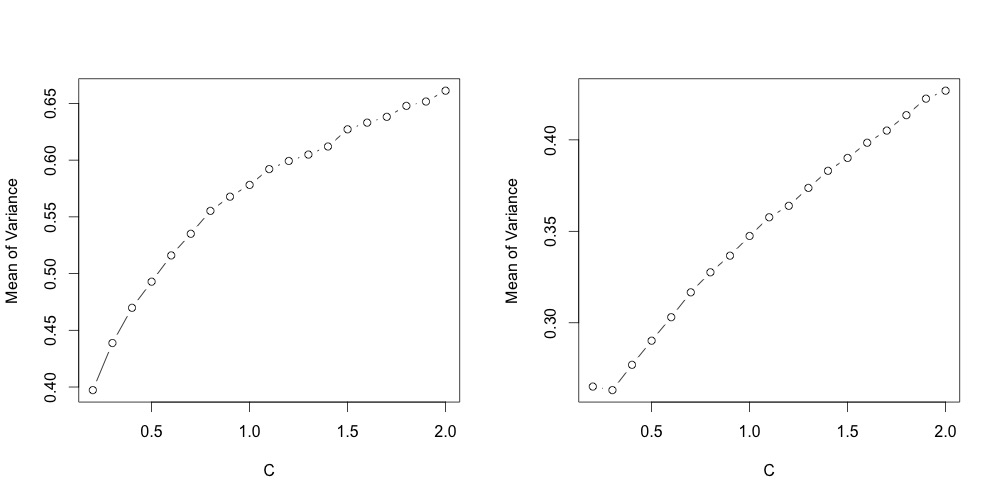
\includegraphics[width=1\linewidth]{abb/c.jpg}
\captionof{figure}{Relation between the variance mean and the regularization parameter $C$. The y-axis represents the mean of the variance of 20 different data sets for each value of $C$(n=100, N=1000).}
\label{fig3}
\end{center}\vspace{1cm}

\subsection*{Influence of the regularization parameter C}
\paragraph{Observations:}
For both Linear and Gaussian Kernel SVMs $C$ is positively correlated with the variance of the SVM-predictions.
\paragraph{Interpretation:}
$C$ controls the trade off between errors of the SVM on training data and margin maximization. To avoid overfitting, the SVM employs regularization and controls the amount of regularization by the constant $C$ (\cite{hastie_elements_2005}). A high value of $C$ corresponds to low regularization, i.e. lower size of slack variables and therefore higher overfitting, which means that the SVM fits the training data too well but does not generalize to new data and therefore the variance of the predictions of our test data rises.


\begin{center}\vspace{1cm}
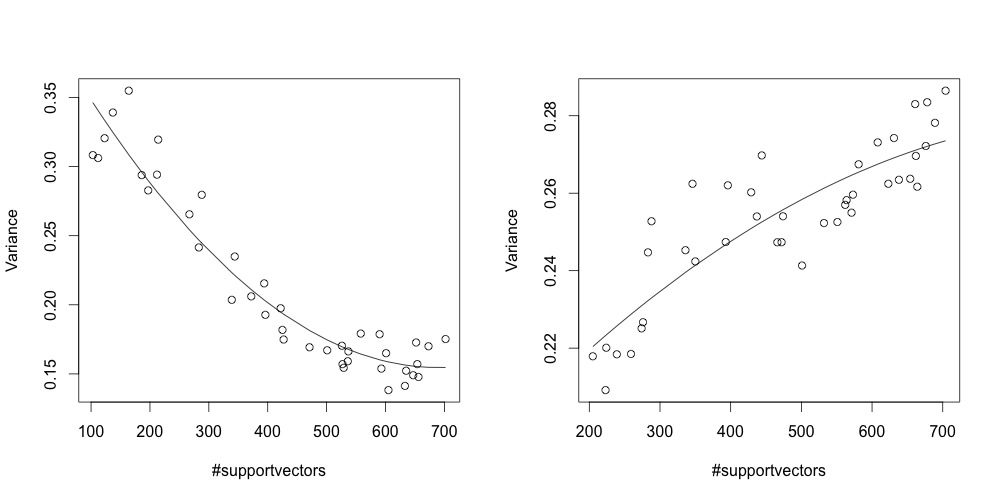
\includegraphics[width=1\linewidth]{abb/n_support.jpg}
\captionof{figure}{Relation between the variance and the number of support vectors( n=1000, N=500)}
\label{fig4}
\end{center}\vspace{1cm}


\subsection*{Influence of the number of support vectors}
\paragraph{Observations:}
The number of support vectors is negatively correlated with the variance of the Linear Kernel and positively correlated with the variance of the Gaussian Kernel.
\paragraph{Interpretation:}
The number of support vectors controls the slack variables of the soft margin SVM. A high number of support vectors implies larger margins and higher slack variables. Training the Linear SVM on the bootstrap samples is therefore more robust and the variance of the decision boundary as well as the distance from each point of the test data set to the decision boundary has smaller variation.
For Gaussian Kernels, a higher number of support vectors might imply overfitting on the training data set and therefore bad generalization to new data which could be the reason why the variance of the predictions of our test data rises.

\begin{center}\vspace{1cm}
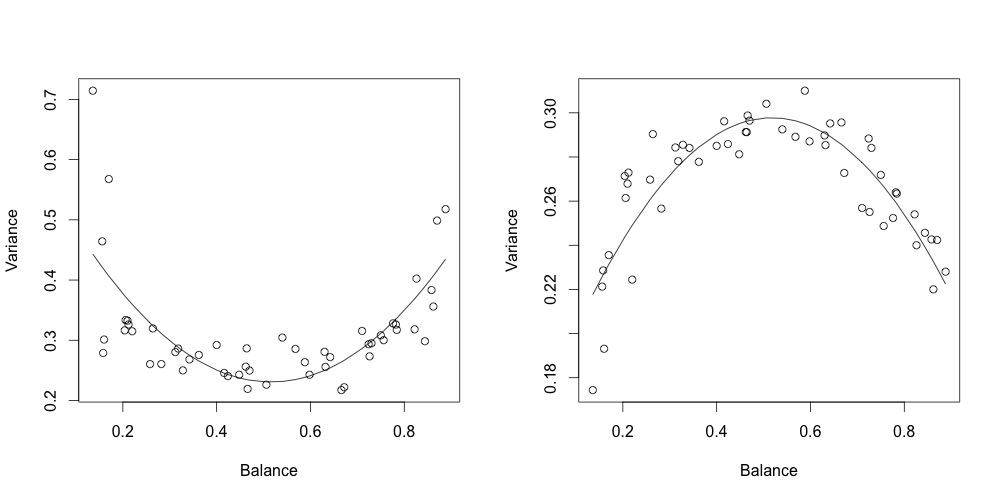
\includegraphics[width=1\linewidth]{abb/balance.jpg}

\captionof{figure}{Relation between variance and balance of the data (n=500, N=1000)}
\label{fig5}
\end{center}\vspace{1cm}



\subsection*{Influence of the balance of the training data set}

\paragraph{Observations:}
Graphs are symmetric around 0.5 for both kernels. For the Linear Kernel, the variance of the SVM rises when the data is unbalanced, it is minimal for perfectly balanced data. For the Gaussian Kernel the maximal variance is attained for perfectly balanced data, it drops for unbalanced data. 
\paragraph{Interpretation:}
In the linear case the variance is especially high, when one class is very small compared to the other class. Depending on which points are sampled from this class, the decision boundary and therefore the distance of test points to this boundary might vary dramatically.
The Gaussian Kernel shows exactly the opposite results. This occurs because the Gaussian Kernel tends to overfit the data on the training data sets (\cite{hastie_elements_2005}). If the data is perfectly balanced, more different samples of the smaller group are possible. Therefore the hyperplanes differ more. If the smaller class is very small, the sample from the smaller class can not differ that much from each other.



%----------------------------------------------------------------------------------------
%	CONCLUSIONS
%----------------------------------------------------------------------------------------

\color{hu_red} % HU red color for the conclusions to make them stand out

\section*{Conclusions}

\begin{itemize}
\item The variance of distances of test points seems to be a good indicator for the robustness of the SVM.
\item The results of changing the $C$-parameter are not surprising but confirm the strength of the variance estimator.
\item Interesting effects of support vectors and data balance.
\item Bootstrapping method has once again shown its value for situations where classical methods of statistical inference are not available.
\end{itemize}

\color{Black} % Set the color back to Black for the rest of the content

%----------------------------------------------------------------------------------------
%	FORTHCOMING RESEARCH
%----------------------------------------------------------------------------------------

 %----------------------------------------------------------------------------------------
%	REFERENCES
%----------------------------------------------------------------------------------------

\nocite{*} % Print all references regardless of whether they were cited in the poster or not
\bibliographystyle{plain} % Plain referencing style
\bibliography{sample} % Use the example bibliography file sample.bib

%----------------------------------------------------------------------------------------
%	ACKNOWLEDGEMENTS
%----------------------------------------------------------------------------------------

%\section*{Acknowledgements}

%Etiam fermentum, arcu ut gravida fringilla, dolor arcu laoreet justo, ut imperdiet urna arcu a arcu. Donec nec ante a dui tempus consectetur. Cras nisi turpis, dapibus sit amet mattis sed, laoreet.

%----------------------------------------------------------------------------------------

\end{multicols}
\end{document}